\documentclass[preprint2]{aastex62}

% CUSTOM PACKAGES AND COMMANDS
% ==============================
% CUSTOM PACKAGES
% =================
\usepackage[shadow]{todonotes}	% \todo{}: side notes at the margins; \todo[inline]{}: inline notes; \missingfigure{}; \listoftodos
\usepackage{color, soul}	% Highlighting, use \hl{...}
\usepackage{wrapfig}	% wrap text around figures; https://en.wikibooks.org/wiki/LaTeX/Floats,_Figures_and_Captions
\usepackage{verbatim}	% comment out chunks of text
\usepackage[normalem]{ulem} % fancy underlining, strikethrough spanning pages. \sout strikethrough, \xout, \underline



% Aliases and new definitions
% =============================

\newcommand{\vdag}{(v)^\dagger}
\newcommand\aastex{AAS\TeX}
\newcommand\latex{La\TeX}

% Symbol: Approximately proportional to (http://tex.stackexchange.com/questions/33538/how-to-get-an-approximately-proportional-to-symbol)
\def\apropto{%
  \def\p{%
    \setbox0=\vbox{\hbox{$\propto$}}%
    \ht0=0.6ex \box0 }%
  \def\s{%
    \vbox{\hbox{$\sim$}}%
  }%
  \mathrel{\raisebox{0.7ex}{%
      \mbox{$\underset{\s}{\p}$}%
    }}%
}

\newcommand{\fermi}{\emph{Fermi}}

\newcommand{\nemmen}{{\bf NEMMEN, R. S.}}

\newcommand{\lat}{\emph{Fermi} LAT Collaboration}

\newcommand{\continue}{\todo[inline,color=RedOrange]{
\centerline{ \textbf{\Large CONTINUE} }   
} }

\newcommand{\mario}{
\begin{wrapfigure}{l}{0.03\textwidth}
\vspace{-20pt}
\begin{center}

\includegraphics[width=0.07\textwidth]{figures/Mario.png}
\end{center}
\vspace{-10pt}
\end{wrapfigure}
}

\newcommand{\bowser}{
\begin{wrapfigure}{l}{0.03\textwidth}
\vspace{-20pt}
\begin{center}
\reflectbox{
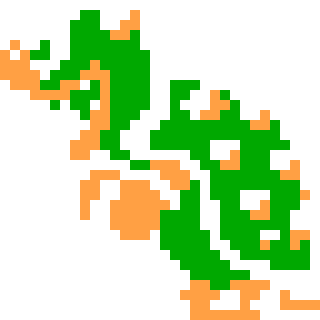
\includegraphics[width=0.07\textwidth]{figures/Bowser.png}
}
\end{center}
\vspace{-10pt}
\end{wrapfigure}
}

% Environment for pretty box with title. Colors inspired
% on default style used in http://www.lasca.ic.unicamp.br/pub/ctan/macros/latex/contrib/tcolorbox/tcolorbox.pdf
% Usage: 
% \begin{boxed}{Box title}
% This is the text formatted by the boxed environment
% \end{boxed}
\definecolor{boxback}{HTML}{DAE5F0}
\definecolor{boxframe}{HTML}{0F365B}
\newenvironment{boxnamed}[1]
{   
\begin{tcolorbox}[enhanced, drop shadow, colframe=boxframe, colback=boxback,title=#1]
}
%text goes here
{
\end{tcolorbox}   
}

% Footnote without marker, cf. http://tex.stackexchange.com/questions/30720/footnote-without-a-marker
\newcommand\orphanfoot[1]{
  \begingroup
  \renewcommand\thefootnote{}\footnote{#1}
  \addtocounter{footnote}{-1}
  \endgroup
}

% figshare
\newcommand{\figshare}{fig\textbf{share}}

% cross (wrong) symbol, needs pifont package
\newcommand{\xmark}{\ding{56}}

% OK symbol (check), needs pifont package
\newcommand{\ok}{\ding{52}}

% Useful for citations with e.g.
\newcommand{\eg}[1]{(e.g. \citealt{#1})}

% fonts for code sample: \code{text sample}
\def\code#1{\texttt{#1}}

% red underline
\def\redul#1{{\color{red} \underline{\color{black}#1}}}







% PAPER PREAMBLE
% ===================
\received{July 1, 2016}
\revised{September 27, 2016}
\accepted{\today}
\submitjournal{ApJ}
%\AuthorCollaborationLimit=3
%% Use \allauthors at the manuscript end to show the full author list.
%% This command should only be used when \AuthorCollaborationLimit is used.

\shorttitle{Spin of M87*}
\shortauthors{Nemmen}
%\watermark{DRAFT} % adds a light gray and diagonal water-mark to the first page. If the text is long you can control the water-mark size with: \setwatermarkfontsize{dimension}






% BEGINNING OF MANUSCRIPT / PAPER CONTENT
% ==========================================
\begin{document}

\title{The spin of M87*}



\correspondingauthor{Rodrigo Nemmen}
\email{rodrigo.nemmen@iag.usp.br}

\author{Rodrigo Nemmen}
\affil{Universidade de S\~ao Paulo, Instituto de Astronomia, Geof\'{\i}sica e Ci\^encias Atmosf\'ericas, Departamento de Astronomia, S\~ao Paulo, SP 05508-090, Brazil}

\begin{comment}
\author{Rodrigo Nemmen}
\affil{Universidade de S\~ao Paulo, Instituto de Astronomia, Geof\'{\i}sica e Ci\^encias Atmosf\'ericas, Departamento de Astronomia, S\~ao Paulo, SP 05508-090, Brazil}
\collaboration{(Fermi LAT Collaboration)}
%\nocollaboration
\end{comment}




\begin{abstract}
By using a combination of observations at different energies: EHT (mass), X-rays, MW (jet power), radio polarization (mdot), we constrain the BH spin of the supermassive black hole at the center of M87, M87*. 
We find that the lower limit on the spin is given by the MAD with beta=1.5. In this case, we find $a/M>0.4$ in the prograde case, and $a/M<-0.5$ in the retrograde case. 
We set limits on the magnetic flux, potentially ruling out some SANE models.
\end{abstract}

\keywords{keywords}





\section{Introduction} \label{sec:intro}

The shadow cast by the event horizon of a black hole (BH) has been imaged for the first time with the Event Horizon Telescope (EHT) for the supermassive black hole (SMBH) at the center of the galaxy M87, known as M87* \citep{EHTC2019}. The observation at a wavelength of 1.3 mm of the asymmetric bright emission ring gives an angular diameter of $d=42 \pm 3 \ \mu$as, which allows an unprecedented constraint on the SMBH mass of $M=(6.5 \pm 0.7) \times 10^9 M_\odot$--the fundamental parameter of the \cite{Kerr1963} metric. The inferred mass is in agreement with--and hence strongly favors--the mass measurement based on stellar dynamics \citep{Gebhardt2011}. 

However, the second fundamental parameter of the Kerr metric--the dimensionless spin $a_* \equiv Jc/GM^2$ where $J$ is the angular momentum of the black hole--is much harder to constrain with shadow observations. The reason is that the ring diameter has a very weak dependence on $a_*$ or the disk inclination, varying by only 4\% in the range $a_*=0$ to $\approx 1$ \citep{Johannsen2010}.

In this Letter, we set bounds on the allowed BH spins of M87* by modeling the energetics of its relativistic jet as being powered by the Blandford-Znajek process--the extraction of BH spin energy through electromagnetic torques. We assume a distance to M87* of 16.8 Mpc \eg{Blakeslee2009, EHTC2019e}. At this distance, cosmological effects are negligible. 



\section{Observations} \label{sec:obs}

Mass accretion rate by \cite{Kuo2014}

Jet power from Cavity power \cite{Russell2013}

?density profile by \cite{Russell2018}?


\section{Models}

, surrounded by a radiatively inefficient accretion flow (RIAF; \citealt{Ichimaru1977, Narayan1994, Yuan2014})

ADIOS \cite{Blandford1999}
need this to connect the Mdot measured by the Faraday rotation with the  BH accretion rate
we keep beta free, allowing for different levels of mass-loss

MAD and SANE models \cite{Narayan2003, Sasha2011, Narayan2012}
describe model
where I take the spin part from? \cite{Sasha2012a}
magnetic flux part
\begin{equation}
\eta = \left( \frac{\phi}{15} \right)^2 % +spin +h/r
\end{equation}

\missingfigure{model efficiency vs a/M, MAD and SANE}




\section{Results} 

\begin{figure}[h]
\centering
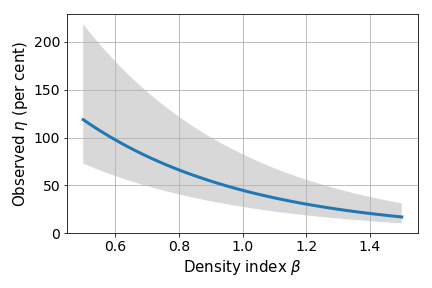
\includegraphics[width=\linewidth]{figures/observed-eta.png}
\caption{empirical jet efficiency for M87* vs beta}
\label{fig:obs-eta}
\end{figure}


\missingfigure{spin MAD (prograde and retrograde) vs beta, taking into account uncertainties on jet power}

\missingfigure{spin vs magnetic flux vs beta (prograde and retrograde), showing some points of particular realizations of MAD and SANE models}




\section{Discussion} \label{sec:disc}

how does this impact the shadow?
connect with Psaltis work
asymmetry on the shadow?

does this rule out any models for consideration, based on the jet energetics?
yes, some magnetic fluxes and spins are ruled out

not all density profiles are allowed in the retrograde case

future constraints with polarimetry




\section{Summary}	\label{sec:summary}

\begin{enumerate}
\item By using a combination of observations at different energies: EHT (mass), X-rays, MW (jet power), radio polarization (mdot), we constrain the BH spin of the supermassive black hole at the center of M87, M87*. 
\item We find that the lower limit on the spin is given by the MAD with beta=1.5. In this case, we find $a/M>0.4$ in the prograde case, and $a/M<-0.5$ in the retrograde case. 
\item We set limits on the magnetic flux, potentially ruling out some SANE models. WHAT LIMITS?
\item density profiles ruled out...
\end{enumerate}






\acknowledgments

We acknowledge useful discussions with Roderik Overzier. This work was supported by FAPESP (Funda\c{c}\~ao de Amparo \`a Pesquisa do Estado de S\~ao Paulo) under grant 2017/01461-2. The Black Hole Group has received a generous donation of a GPU from NVIDIA under the GPU Grant Program.

\vspace{5mm}
\facilities{Fermi LAT}
\software{astropy \citep{astropy}, \href{http://pandas.pydata.org/index.html}{Pandas}, Jupyter \citep{ipython}.} % specifies which programs were used



\appendix

\section{Appendix information}



% REFERENCES
% ============
\bibliography{refs}

%\allauthors % shows entire author+affilation list. Has to go at the end of the manuscript

%% Include this line if you are using the \added, \replaced, \deleted
%% commands to see a summary list of all changes at the end of the article.
%\listofchanges

\end{document}